% Created by tikzDevice version 0.12.3 on 2020-09-29 12:05:42
% !TEX encoding = UTF-8 Unicode
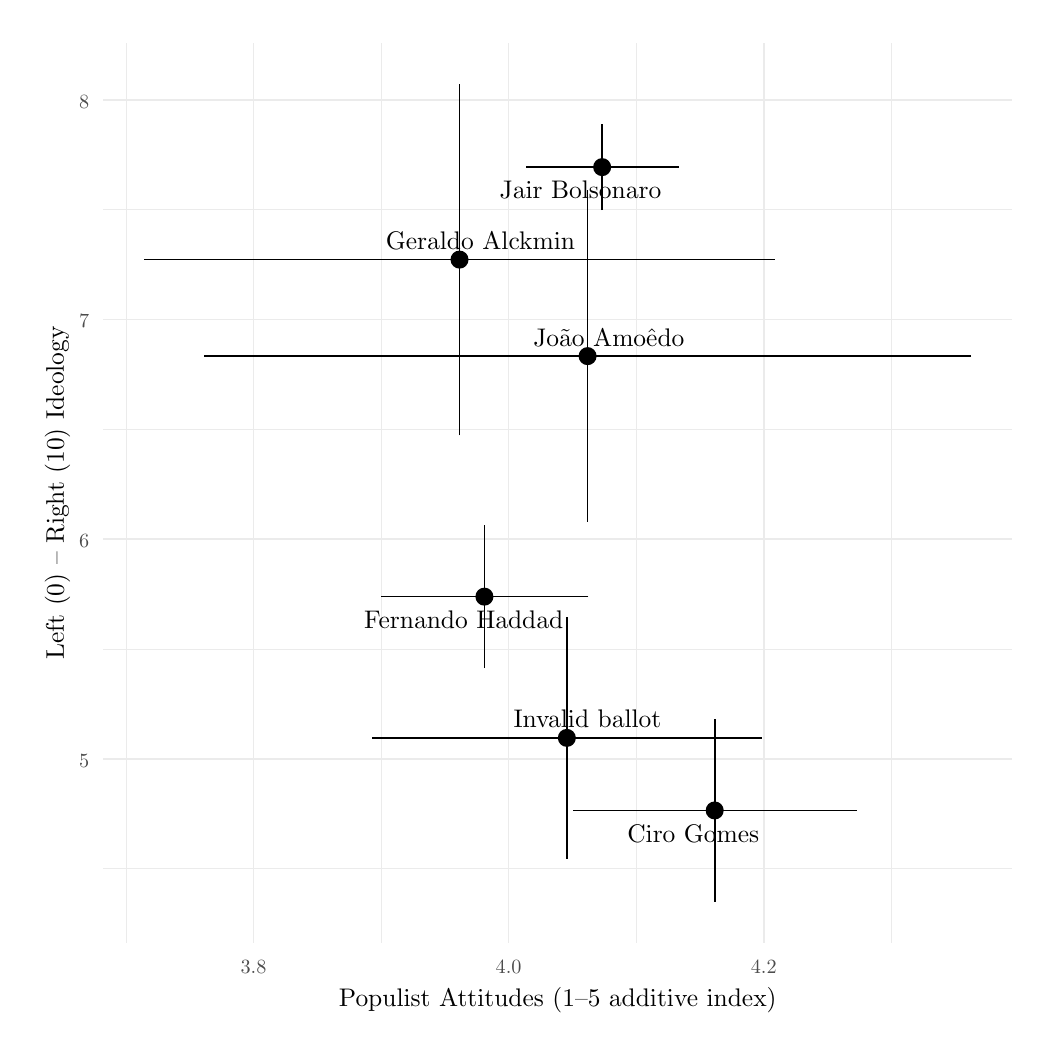
\begin{tikzpicture}[x=1pt,y=1pt]
\definecolor{fillColor}{RGB}{255,255,255}
\path[use as bounding box,fill=fillColor,fill opacity=0.00] (0,0) rectangle (361.35,361.35);
\begin{scope}
\path[clip] ( 27.22, 30.69) rectangle (355.85,355.85);
\definecolor{drawColor}{gray}{0.92}

\path[draw=drawColor,line width= 0.3pt,line join=round] ( 27.22, 57.41) --
	(355.85, 57.41);

\path[draw=drawColor,line width= 0.3pt,line join=round] ( 27.22,136.80) --
	(355.85,136.80);

\path[draw=drawColor,line width= 0.3pt,line join=round] ( 27.22,216.19) --
	(355.85,216.19);

\path[draw=drawColor,line width= 0.3pt,line join=round] ( 27.22,295.58) --
	(355.85,295.58);

\path[draw=drawColor,line width= 0.3pt,line join=round] ( 35.50, 30.69) --
	( 35.50,355.85);

\path[draw=drawColor,line width= 0.3pt,line join=round] (127.69, 30.69) --
	(127.69,355.85);

\path[draw=drawColor,line width= 0.3pt,line join=round] (219.88, 30.69) --
	(219.88,355.85);

\path[draw=drawColor,line width= 0.3pt,line join=round] (312.07, 30.69) --
	(312.07,355.85);

\path[draw=drawColor,line width= 0.6pt,line join=round] ( 27.22, 97.11) --
	(355.85, 97.11);

\path[draw=drawColor,line width= 0.6pt,line join=round] ( 27.22,176.50) --
	(355.85,176.50);

\path[draw=drawColor,line width= 0.6pt,line join=round] ( 27.22,255.89) --
	(355.85,255.89);

\path[draw=drawColor,line width= 0.6pt,line join=round] ( 27.22,335.28) --
	(355.85,335.28);

\path[draw=drawColor,line width= 0.6pt,line join=round] ( 81.59, 30.69) --
	( 81.59,355.85);

\path[draw=drawColor,line width= 0.6pt,line join=round] (173.78, 30.69) --
	(173.78,355.85);

\path[draw=drawColor,line width= 0.6pt,line join=round] (265.97, 30.69) --
	(265.97,355.85);
\definecolor{drawColor}{RGB}{0,0,0}

\path[draw=drawColor,line width= 0.6pt,line join=round] (248.25, 45.47) -- (248.25,111.51);

\path[draw=drawColor,line width= 0.6pt,line join=round] (165.04,129.90) -- (165.04,181.60);

\path[draw=drawColor,line width= 0.6pt,line join=round] (156.05,214.01) -- (156.05,341.07);

\path[draw=drawColor,line width= 0.6pt,line join=round] (194.83, 61.11) -- (194.83,148.31);

\path[draw=drawColor,line width= 0.6pt,line join=round] (207.59,295.43) -- (207.59,326.50);

\path[draw=drawColor,line width= 0.6pt,line join=round] (202.32,182.81) -- (202.32,302.51);
\definecolor{fillColor}{RGB}{0,0,0}

\path[draw=drawColor,line width= 0.8pt,line join=round,line cap=round,fill=fillColor] (248.25, 78.49) circle (  2.85);

\path[draw=drawColor,line width= 0.8pt,line join=round,line cap=round,fill=fillColor] (165.04,155.75) circle (  2.85);

\path[draw=drawColor,line width= 0.8pt,line join=round,line cap=round,fill=fillColor] (156.05,277.54) circle (  2.85);

\path[draw=drawColor,line width= 0.8pt,line join=round,line cap=round,fill=fillColor] (194.83,104.71) circle (  2.85);

\path[draw=drawColor,line width= 0.8pt,line join=round,line cap=round,fill=fillColor] (207.59,310.96) circle (  2.85);

\path[draw=drawColor,line width= 0.8pt,line join=round,line cap=round,fill=fillColor] (202.32,242.66) circle (  2.85);

\path[draw=drawColor,line width= 0.6pt,line join=round] (299.59, 78.49) --
	(299.59, 78.49);

\path[draw=drawColor,line width= 0.6pt,line join=round] (299.59, 78.49) --
	(196.92, 78.49);

\path[draw=drawColor,line width= 0.6pt,line join=round] (196.92, 78.49) --
	(196.92, 78.49);

\path[draw=drawColor,line width= 0.6pt,line join=round] (202.59,155.75) --
	(202.59,155.75);

\path[draw=drawColor,line width= 0.6pt,line join=round] (202.59,155.75) --
	(127.50,155.75);

\path[draw=drawColor,line width= 0.6pt,line join=round] (127.50,155.75) --
	(127.50,155.75);

\path[draw=drawColor,line width= 0.6pt,line join=round] (269.95,277.54) --
	(269.95,277.54);

\path[draw=drawColor,line width= 0.6pt,line join=round] (269.95,277.54) --
	( 42.16,277.54);

\path[draw=drawColor,line width= 0.6pt,line join=round] ( 42.16,277.54) --
	( 42.16,277.54);

\path[draw=drawColor,line width= 0.6pt,line join=round] (265.30,104.71) --
	(265.30,104.71);

\path[draw=drawColor,line width= 0.6pt,line join=round] (265.30,104.71) --
	(124.36,104.71);

\path[draw=drawColor,line width= 0.6pt,line join=round] (124.36,104.71) --
	(124.36,104.71);

\path[draw=drawColor,line width= 0.6pt,line join=round] (235.25,310.96) --
	(235.25,310.96);

\path[draw=drawColor,line width= 0.6pt,line join=round] (235.25,310.96) --
	(179.93,310.96);

\path[draw=drawColor,line width= 0.6pt,line join=round] (179.93,310.96) --
	(179.93,310.96);

\path[draw=drawColor,line width= 0.6pt,line join=round] (340.91,242.66) --
	(340.91,242.66);

\path[draw=drawColor,line width= 0.6pt,line join=round] (340.91,242.66) --
	( 63.72,242.66);

\path[draw=drawColor,line width= 0.6pt,line join=round] ( 63.72,242.66) --
	( 63.72,242.66);

\node[text=drawColor,anchor=base,inner sep=0pt, outer sep=0pt, scale=  0.92] at (240.51, 66.92) {Ciro Gomes};

\node[text=drawColor,anchor=base,inner sep=0pt, outer sep=0pt, scale=  0.92] at (157.55,144.37) {Fernando Haddad};

\node[text=drawColor,anchor=base,inner sep=0pt, outer sep=0pt, scale=  0.92] at (163.61,281.36) {Geraldo Alckmin};

\node[text=drawColor,anchor=base,inner sep=0pt, outer sep=0pt, scale=  0.92] at (202.26,108.37) {Invalid ballot};

\node[text=drawColor,anchor=base,inner sep=0pt, outer sep=0pt, scale=  0.92] at (199.76,299.57) {Jair Bolsonaro};

\node[text=drawColor,anchor=base,inner sep=0pt, outer sep=0pt, scale=  0.92] at (210.03,246.28) {João Amoêdo};
\end{scope}
\begin{scope}
\path[clip] (  0.00,  0.00) rectangle (361.35,361.35);
\definecolor{drawColor}{gray}{0.30}

\node[text=drawColor,anchor=base east,inner sep=0pt, outer sep=0pt, scale=  0.73] at ( 22.27, 94.08) {5};

\node[text=drawColor,anchor=base east,inner sep=0pt, outer sep=0pt, scale=  0.73] at ( 22.27,173.47) {6};

\node[text=drawColor,anchor=base east,inner sep=0pt, outer sep=0pt, scale=  0.73] at ( 22.27,252.86) {7};

\node[text=drawColor,anchor=base east,inner sep=0pt, outer sep=0pt, scale=  0.73] at ( 22.27,332.25) {8};
\end{scope}
\begin{scope}
\path[clip] (  0.00,  0.00) rectangle (361.35,361.35);
\definecolor{drawColor}{gray}{0.30}

\node[text=drawColor,anchor=base,inner sep=0pt, outer sep=0pt, scale=  0.73] at ( 81.59, 19.68) {3.8};

\node[text=drawColor,anchor=base,inner sep=0pt, outer sep=0pt, scale=  0.73] at (173.78, 19.68) {4.0};

\node[text=drawColor,anchor=base,inner sep=0pt, outer sep=0pt, scale=  0.73] at (265.97, 19.68) {4.2};
\end{scope}
\begin{scope}
\path[clip] (  0.00,  0.00) rectangle (361.35,361.35);
\definecolor{drawColor}{RGB}{0,0,0}

\node[text=drawColor,anchor=base,inner sep=0pt, outer sep=0pt, scale=  0.92] at (191.54,  7.64) {Populist Attitudes (1--5 additive index)};
\end{scope}
\begin{scope}
\path[clip] (  0.00,  0.00) rectangle (361.35,361.35);
\definecolor{drawColor}{RGB}{0,0,0}

\node[text=drawColor,rotate= 90.00,anchor=base,inner sep=0pt, outer sep=0pt, scale=  0.92] at ( 13.08,193.27) {Left (0) -- Right (10) Ideology};
\end{scope}
\end{tikzpicture}
